\documentclass{standalone}
\usepackage{tikz}
\usetikzlibrary{decorations.pathreplacing,calc}
\begin{document}
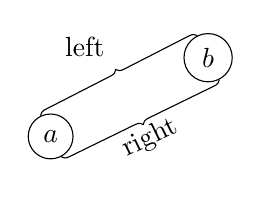
\begin{tikzpicture}

\newcommand{\bracket}[3]{
    \draw[decorate,decoration=brace]
      let
        \p1 = ($(#2)-(#1)$),
        \n{angle} = {atan2(\y1,\x1)+90}
      in
        (#1.\n{angle}) --#3 (#2.\n{angle});
}

\node[draw,circle] (a) at (0,0) {$a$};
\node[draw,circle] (b) at (2,1) {$b$};

\bracket{a}{b}{node[label=\n{angle}:left]{}}
\bracket{b}{a}{node[sloped,below]{right}}

\end{tikzpicture}
\end{document}
